% ============================================================
%  SCHOLA DOMESTICA — Magister Mathematica
%  Level 1 | Week 11 | Day 2
%  Topic: Addition Facts — +8, +9, and 5+5=10
% ============================================================
\documentclass[12pt, letterpaper]{article}

\usepackage[top=1in, bottom=1in, left=1in, right=1in]{geometry}
\usepackage[T1]{fontenc}
\usepackage[utf8]{inputenc}
\usepackage{lmodern}
\usepackage{microtype}
\usepackage{amsmath}
\usepackage{xcolor}
\usepackage{tikz}
\usepackage{array}
\usepackage{enumitem}
\usepackage{multicol}
\usepackage{mdframed}
\usepackage{fancyhdr}

\definecolor{scholared}{RGB}{160,30,30}
\definecolor{scholagold}{RGB}{180,140,40}
\definecolor{scholacream}{RGB}{253,248,235}
\definecolor{scholagreen}{RGB}{50,110,60}
\definecolor{scholablue}{RGB}{40,80,140}

\pagestyle{fancy}
\fancyhf{}
\renewcommand{\headrulewidth}{0.6pt}
\fancyhead[L]{\small\textcolor{scholared}{\textbf{Schola Domestica — Magister Mathematica}}}
\fancyhead[R]{\small\textcolor{scholared}{Level 1 · Week 11 · Day 2}}
\fancyfoot[C]{\small\textcolor{gray}{— \thepage\ —}}

\newcommand{\answerline}{\underline{\hspace{2.5cm}}}
\newcommand{\biganswerline}{\underline{\hspace{4cm}}}
\newcommand{\numbox}{\tikz{\draw[scholablue,thick](0,0)rectangle(1.2cm,0.85cm);}}

\newmdenv[
  backgroundcolor=scholacream,
  linecolor=scholared,
  linewidth=1.5pt,
  roundcorner=6pt,
  innertopmargin=8pt,
  innerbottommargin=8pt,
  innerleftmargin=10pt,
  innerrightmargin=10pt
]{lessonbox}

\newmdenv[
  backgroundcolor={rgb,255:red,235;green,245;blue,235},
  linecolor=scholagreen,
  linewidth=1.2pt,
  roundcorner=4pt,
  innertopmargin=6pt,
  innerbottommargin=6pt,
  innerleftmargin=8pt,
  innerrightmargin=8pt
]{enrichbox}

\begin{document}

\begin{center}
  {\LARGE\textbf{\textcolor{scholared}{Adding Eight, Nine, and Ten:}}}\\[4pt]
  {\Large\textcolor{scholagold}{\textit{The Last Facts to Ten}}}\\[6pt]
  {\small Name: \biganswerline \hspace{1cm} Date: \answerline}
\end{center}

\vspace{4pt}
\noindent\textcolor{scholared}{\rule{\linewidth}{1pt}}
\vspace{4pt}

% IMAGE PROMPT (Beatrix Potter watercolour style):
% Two squirrels each hold five acorns — one on each side of a mossy oak stump. Together they
% tip them onto the stump to make one pile of ten. Warm autumn palette, no text.

\begin{lessonbox}
\textbf{Special trick for $+9$:} Adding 9 is the same as adding 10 and taking away 1.\\[4pt]
\hspace{1em} $2 + 9$: think ``$2 + 10 = 12$, then back one: \textbf{11}''\\[6pt]
\textbf{Double 5:} $5 + 5 = \mathbf{10}$ — two hands together!\\
\hspace{1em} This is the biggest doubles fact to 10. Memorise it!
\end{lessonbox}

\bigskip

% Number line 0–10
\noindent
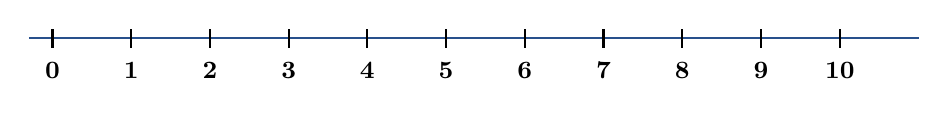
\begin{tikzpicture}
  \draw[thick, scholablue] (0,0) -- (11.3,0);
  \foreach \n in {0,...,10} {
    \draw[thick] (\n*1.0+0.3, -0.12) -- (\n*1.0+0.3, 0.12);
    \node[below] at (\n*1.0+0.3, -0.18) {\small\textbf{\n}};
  }
\end{tikzpicture}

\bigskip

% ===== PART I: +8 FACTS =====
\noindent\textcolor{scholared}{\large\textbf{Part I — Adding Eight}} \hfill \textit{(Problems 1–4)}

\bigskip

\noindent
\begin{tabular}{@{}p{3.5cm} p{3.5cm} p{3.5cm} p{3.5cm}@{}}
\textbf{1.}\; $0 + 8 =$ \numbox &
\textbf{2.}\; $1 + 8 =$ \numbox &
\textbf{3.}\; $2 + 8 =$ \numbox &
\textbf{4.}\; $8 + 2 =$ \numbox
\end{tabular}

\medskip
\noindent\textit{Problems 3 and 4: Do they give the same sum? \quad $\square$ Yes \quad $\square$ No}

\bigskip\bigskip

% ===== PART II: +9 WITH THE TRICK =====
\noindent\textcolor{scholared}{\large\textbf{Part II — Adding Nine (the $+10$ trick)}} \hfill \textit{(Problems 5–8)}

\medskip
\noindent\textit{Fill in both steps.}

\bigskip

\noindent\textbf{5.} $1 + 10 =$ \numbox \quad so $1 + 9 =$ \numbox

\medskip
\noindent\textbf{6.} $0 + 10 =$ \numbox \quad so $0 + 9 =$ \numbox

\medskip
\noindent\textbf{7.} $9 + 1 =$ \numbox \quad (\textit{turn-around of problem 5})

\medskip
\noindent\textbf{8.} $9 + 0 =$ \numbox

\bigskip\bigskip

% ===== PART III: DOUBLE 5+5 AND FRIENDS =====
\noindent\textcolor{scholared}{\large\textbf{Part III — Five and Five}} \hfill \textit{(Problems 9–12)}

\bigskip

\noindent\textbf{9.}\; $5 + 5 =$ \numbox \quad \textit{(two whole hands!)}

\medskip
\noindent
\begin{tabular}{@{}p{7.0cm} p{7.0cm}@{}}
\textbf{10.}\; $5 + 4 =$ \numbox &
\textbf{11.}\; $4 + 5 =$ \numbox
\end{tabular}

\medskip
\noindent\textbf{12.}\; Do problems 10 and 11 give the same answer? \quad $\square$ Yes \quad $\square$ No \quad Because: \answerline

\bigskip\bigskip

% ===== PART IV: MIXED TO 10 =====
\noindent\textcolor{scholared}{\large\textbf{Part IV — Mixed Facts: All Sums to 10}} \hfill \textit{(Problems 13–16)}

\bigskip

\noindent
\begin{tabular}{@{}p{3.5cm} p{3.5cm} p{3.5cm} p{3.5cm}@{}}
\textbf{13.}\; $6 + 4 =$ \numbox &
\textbf{14.}\; $7 + 3 =$ \numbox &
\textbf{15.}\; $8 + 2 =$ \numbox &
\textbf{16.}\; $9 + 1 =$ \numbox
\end{tabular}

\bigskip

\begin{enrichbox}
\textbf{\textcolor{scholagreen}{The Ten-Pairs — complete them all!}}\\[4pt]
$\mathbf{0}+10=10$ \quad $\mathbf{1}+9=10$ \quad $\mathbf{2}+8=10$ \quad $\mathbf{3}+7=10$ \quad $\mathbf{4}+6=10$ \quad $\mathbf{5}+5=10$\\[3pt]
\textit{Can you say the whole list without looking? These are some of the most useful facts in all of arithmetic!}
\end{enrichbox}

\vspace{0.3cm}
\noindent\textcolor{gray}{\small\textit{Ray's Primary Arithmetic — the $+9$ trick and ten-pairs.}}

\end{document}
